\documentclass[11pt,a4paper]{article}

\usepackage[margin=1in]{geometry}
\usepackage[T1]{fontenc}
\usepackage{lmodern}
\usepackage{microtype}
\usepackage{amsmath}
\usepackage{booktabs}
\usepackage{longtable}
\usepackage{tabularx}
\usepackage{array}
\usepackage{graphicx}
\usepackage{float}
\usepackage{enumitem}
\usepackage{xcolor}
\usepackage{listings}
\usepackage[numbers,sort&compress]{natbib}
\usepackage[hidelinks]{hyperref}

\graphicspath{{../../results/C_final/figures/}}

\definecolor{codegray}{gray}{0.95}
\lstset{
  basicstyle=\ttfamily\small,
  backgroundcolor=\color{codegray},
  frame=single,
  breaklines=true,
  columns=fullflexible,
  keepspaces=true
}

\newcommand{\Fone}{macro-F1}
\newcommand{\Dropout}{\textit{Dropout}}
\newcommand{\Enrolled}{\textit{Enrolled}}
\newcommand{\Graduate}{\textit{Graduate}}

\title{Predicting Student Dropout and Academic Success\\
\large A comparison of enrolment and first-semester information}
\author{%
  Ruxuan ZHOU \and Mingxi ZHU \and Boyi WEI \and Mengqi YAN \and Yushu WU\\[4pt]
  \normalsize Group: Zero Bias Hero\quad DSC5001 Group Project
}
\date{November 2026}

\begin{document}

\maketitle

\begin{abstract}
When a student is at risk of dropping out, an institution needs to know early enough to help.
This report asks a concrete question: how much does adding first-semester academic records to
enrolment-time information improve the classification of students as \Dropout{}, \Enrolled{},
or \Graduate{}? The answer determines whether waiting a full term for first-semester data
is worth the delay.

Using 4,424 records from a Portuguese polytechnic (2008--2019), we train logistic regression,
decision tree, and random forest models under two feature sets (18 enrolment variables; 24
variables adding six first-semester academic measures) with a fixed stratified split and
five-fold cross-validation. The representative model for interpretation is pre-specified before
any test data is seen, and the held-out test set is used exactly once.

First-semester information raises test macro-F1 by 0.125--0.142 across every model family and
substantially improves Dropout detection. The key signal is not grades alone but the gap between
units enrolled and units approved: students who register for many units but convert few are the
ones reliably flagged. Logistic regression performs at least as well as the random forest on the
richer feature set (macro-F1 0.6442 vs 0.6153), which favours the more interpretable model.
The \Enrolled{} class remains the persistent weak point across all models.

These results support a retrospective end-of-first-semester screening workflow. Deployment
requires human review, non-punitive intervention design, and fairness monitoring.
\end{abstract}

\noindent\textbf{Keywords:} student dropout, academic success, multiclass classification,
macro-F1, early support, reproducible machine learning

\tableofcontents
\newpage

\section{Introduction}

Students drop out for many reasons, and institutions cannot help everyone at once. The practical
question is who to contact and when. Predictive models can help prioritise that outreach, but
they are only useful when they are evaluated honestly. A model that simply predicts \Graduate{}
for everyone reaches 50\% accuracy on this dataset while detecting zero dropouts.

This project asks how much adding first-semester academic records to enrolment-time information
actually changes prediction quality. The question has a real cost attached: first-semester data
requires waiting a full term, which delays any intervention. If the gain is modest, enrolment-only
screening may be sufficient. If it is large, the wait is justified.

\subsection{What prior work leaves open}

Studies on student dropout prediction often report accuracy above 80\%
\citep{berens2019,aulck2016}. These figures are frequently misleading for three reasons. First,
many studies collapse the three natural outcome classes (\Dropout{}, still-\Enrolled{},
\Graduate{}) into a binary problem \citep{marbouti2016}, hiding the difficulty of distinguishing
students who are still progressing from those who have already left. Second, accuracy rewards
majority-class prediction; a balanced metric like macro-F1 \citep{sokolova2009} exposes poor
minority-class performance where accuracy conceals it. Third, few studies pre-specify which model
will be used for interpretation before looking at test results, leaving open the possibility of
picking whichever model happened to score highest.

The information-timing comparison is also rarely clean. Studies that contrast ``enrolment only''
versus ``enrolment plus early academic performance'' often do not document precisely which
variables belong to which information point, so it is unclear whether the comparison supports a
real-time alert or only a retrospective review.

\subsection{Our approach}

We ran a controlled experiment on the UCI dataset ``Predict Students' Dropout and Academic
Success'' \citep{realinho2021}: 4,424 students from a single Portuguese polytechnic, 2008--2019,
with three outcome classes retained as labelled. The design has four properties worth noting:

\begin{enumerate}[leftmargin=*]
  \item \textbf{Three-class outcome, balanced metric.} We retain \Dropout{}, \Enrolled{}, and
  \Graduate{} and select models by macro-F1, which weights each class equally. This forces the
  evaluation to confront how hard the middle class is rather than averaging over it.

  \item \textbf{Clean information boundary.} Feature set 1 contains the 18 variables available
  at enrolment. Feature set 2 adds six first-semester academic measures. Second-semester
  variables and fields with uncertain measurement timing are excluded, keeping the two conditions
  genuinely comparable.

  \item \textbf{Pre-specified interpretation model.} The 24-variable random forest was fixed as
  the representative model based on cross-validation alone, before any test score was computed.
  It is not changed even when test results favour another model.

  \item \textbf{One-shot test evaluation.} Hyperparameter tuning uses only the training partition.
  The held-out test set is applied exactly once, after all models are frozen.
\end{enumerate}

\subsection{Research questions}

\begin{enumerate}[leftmargin=*]
  \item How much does adding first-semester academic information improve prediction over
  enrolment information alone?
  \item Do simpler models (logistic regression) perform as well as more complex ones (random
  forest), and do validation rankings survive to the test set?
  \item Which features and classes determine whether the models are usable for a support
  screening workflow?
\end{enumerate}

\subsection{Team workflow}

Work was divided into four sequential stages. Ruxuan ZHOU (Member A) prepared the data and fixed
the split and feature definitions. Mingxi ZHU (Member B) tuned and froze six model pipelines plus
a majority-class baseline. Boyi WEI (Member C) applied those frozen pipelines once to the
held-out test rows and produced the final metrics, predictions, figures, and interpretation
tables. Mengqi YAN (Member D) integrates those materials into this report. Yushu WU (Member E)
will prepare the presentation slides and recording. A full contribution breakdown is in
Appendix~\ref{app:contributions}.

\section{Data and experimental protocol}

\subsection{Data source and outcome}

The source is the UCI Machine Learning Repository dataset by Realinho et al.\ \citep{realinho2021}.
It contains 4,424 student records from a Portuguese polytechnic, covering enrolments from 2008 to
2019. The data are administrative enrolment and academic records with minimal missing values.
Categorical variables (marital status, application mode, course, etc.) and numerical variables
(admission grade, age, previous qualification grade) are complete as recorded by the institution's
registration system.

\textbf{Outcome definition.} The outcome is a three-class label assigned at the institutional level:
\begin{itemize}[leftmargin=*]
  \item \textbf{\Dropout{}}: Student left this programme or institution without completing the degree.
  \item \textbf{\Enrolled{}}: Student was still enrolled at the time of data collection.
  \item \textbf{\Graduate{}}: Student completed all degree requirements.
\end{itemize}

The \Dropout{} label is institution-specific. A student recorded as Dropout may have transferred to
another programme or institution and graduated there; the label tracks outcome at this institution,
not lifetime educational attainment. \Enrolled{} is a temporary state captured at data collection:
some students in this category will eventually graduate, others will eventually drop out.

\textbf{Data preparation.} Member A retained the raw file without changing predictor values. A
stable \texttt{row\_id} identifier was assigned before column-name trimming, and the prepared
file contains all 4,424 records. The outcome distribution in the held-out test set is 284
\Dropout{} (32.1\%), 159 \Enrolled{} (18.0\%), and 442 \Graduate{} (49.9\%). A classifier that
always predicts \Graduate{} obtains 0.4994 accuracy on this split, so accuracy alone would conceal
poor performance on the minority classes.

This dataset comes from one Portuguese polytechnic over 2008--2019 cohorts. The results should
not be assumed to transfer to research universities (different student profiles), other countries
(different education systems), or recent cohorts affected by the COVID-19 pandemic (2020 onward).

\subsection{Fixed split and leakage controls}

The protocol fixes random seed 42, a stratified 80/20 outer split, and five stratified folds
within the training portion. The resulting sample sizes are 3,539 training rows and 885 test
rows. The split manifest stores \texttt{row\_id}, \texttt{dataset\_split}, and \texttt{cv\_fold};
the test rows have no cross-validation fold. All learned preprocessing is fitted inside each
training fold, and the test rows are not used for feature selection, hyperparameter tuning,
threshold changes, or model selection.

The primary selection metric is macro-F1:
\begin{equation}
  \mathrm{macro\mbox{-}F1} = \frac{1}{3}\sum_{c\in\{\Dropout,\Enrolled,\Graduate\}}
  \mathrm{F1}_c,
\end{equation}
which gives each class equal weight. Dropout precision and recall are reported as operational
secondary measures. This choice is appropriate because the Graduate class is the largest and
because a support intervention should not be evaluated only by its performance on that class.

\subsection{Feature sets}

The first feature set contains 18 variables available at enrolment. The second contains those
18 variables plus six first-semester academic variables. The project excludes second-semester
variables, fields with uncertain measurement timing, and macroeconomic variables whose
availability at enrolment is not sufficiently documented. Target, row identifiers, split labels,
and fold labels are never predictors.

\begin{table}[H]
\centering
\caption{Feature sets used in the fixed experiment.}
\label{tab:features}
\begin{tabularx}{\textwidth}{>{\raggedright\arraybackslash}p{0.28\textwidth}X}
\toprule
Feature set & Variables \\
\midrule
Enrolment (18) & Marital status; application mode and order; course; attendance; previous
qualification and grade; nationality; parents' qualification and occupation; admission grade;
displacement; educational special needs; gender; age at enrolment; international status. \\
Enrolment + first semester (24) & All 18 enrolment variables, plus credited, enrolled,
evaluated, and approved curricular units; first-semester grade; and units without evaluations. \\
\bottomrule
\end{tabularx}
\end{table}

\section{Models and reproducibility}

\subsection{Model selection rationale}

We compared three model families that sit at different points on the complexity-interpretability
spectrum \citep{hastie2009}:

\begin{enumerate}[leftmargin=*]
  \item \textbf{Logistic regression.} A linear model with signed coefficients for each feature.
  Straightforward to interpret and to explain to a non-technical audience. Limited to linear
  decision boundaries.

  \item \textbf{Decision tree.} Learns axis-aligned splits and can be read as an explicit rule
  set. Captures non-linear patterns without manual feature engineering, but prone to overfitting
  without depth constraints.

  \item \textbf{Random forest.} An ensemble of decision trees \citep{breiman2001} that averages
  out the variance of individual trees. More robust than a single tree, and permutation importance
  \citep{strobl2008} provides a feature ranking. Individual decisions are harder to trace than in
  the other two models.
\end{enumerate}

We did not include neural networks (the dataset has 4,424 rows, which is small for deep learning),
support vector machines (similar performance to logistic regression in preliminary tests with
reduced interpretability), or gradient boosting (the added complexity was not warranted given the
project scope).

\subsection{Feature engineering and preprocessing}

The dataset contains 14 categorical variables (marital status, application mode, course,
attendance, previous qualification, nationality, parents' qualification and occupation, gender,
international status) and 10 numerical variables (age, admission grade, previous qualification
grade, six first-semester academic metrics). All preprocessing is fitted separately within each
cross-validation fold to prevent leakage from validation data into the training step.

Categorical variables are encoded with one-hot encoding. Numerical variables are standardised
with \texttt{StandardScaler} (zero mean, unit variance) fitted on the training fold and applied
to validation and test data. No polynomial features or interaction terms were added manually;
tree-based models pick up interactions through their splitting structure, while logistic
regression sees only the raw linear combination.

\subsection{Hyperparameter tuning}

Member B ran a grid search over hyperparameters using five-fold cross-validation on the 3,539
training rows, selecting the configuration with the highest mean macro-F1. The search spaces and
chosen values were:

\textbf{Logistic regression:}
\begin{itemize}[leftmargin=*]
  \item Regularisation strength $C$: \{0.001, 0.01, 0.1, 1.0, 10.0\}; class weight: \{None, balanced\}
  \item Chosen for 18-variable set: $C=0.1$, balanced class weights
  \item Chosen for 24-variable set: $C=1.0$, balanced class weights
\end{itemize}

\textbf{Decision tree:}
\begin{itemize}[leftmargin=*]
  \item Maximum depth: \{3, 6, 9, 12, None\}; min samples per leaf: \{1, 5, 10, 20\}; class weight: \{None, balanced\}
  \item Chosen for 18-variable set: unconstrained depth, min leaf 20, balanced weights
  \item Chosen for 24-variable set: max depth 6, min leaf 20, no class weighting
\end{itemize}

\textbf{Random forest:}
\begin{itemize}[leftmargin=*]
  \item Trees: fixed at 100; max depth: \{6, 9, 12, None\}; min samples per leaf: \{1, 5, 10\}; class weight: \{None, balanced\}
  \item Chosen for 18-variable set: max depth 12, min leaf 1, balanced weights
  \item Chosen for 24-variable set: unconstrained depth, min leaf 1, balanced weights
\end{itemize}

Balanced class weighting was selected for most models, reflecting the skewed outcome distribution
(50\% Graduate, 32\% Dropout, 18\% Enrolled). The full search covered 52 candidate configurations
across all three model families and both feature sets.

\subsection{Model freezing and representative selection}

After hyperparameter selection, Member B refitted each chosen configuration on the full 3,539
training rows and saved the pipelines. The 24-variable random forest was fixed as the
representative model for interpretation at this point, based solely on its cross-validation score.
The cross-validation results are in Table~\ref{tab:cv}.

\begin{table}[H]
\centering
\caption{Training-only cross-validation results reported by Member B. Values are mean macro-F1
with fold standard deviation.}
\label{tab:cv}
\begin{tabular}{llr}
\toprule
Feature set & Model & CV macro-F1 \\
\midrule
Enrolment & Logistic regression & 0.5235 $\pm$ 0.0100 \\
Enrolment & Decision tree & 0.4552 $\pm$ 0.0342 \\
Enrolment & Random forest & 0.5190 $\pm$ 0.0085 \\
Enrolment + first semester & Logistic regression & 0.6444 $\pm$ 0.0159 \\
Enrolment + first semester & Decision tree & 0.6016 $\pm$ 0.0141 \\
Enrolment + first semester & Random forest & 0.6449 $\pm$ 0.0172 \\
Majority baseline & Most frequent class & 0.2220 $\pm$ 0.0002 \\
\bottomrule
\end{tabular}
\end{table}

The random forest using the 24-variable feature set was fixed as the representative model before
Member C ran any test evaluation. It is kept as the representative model throughout this report
even though the test results put logistic regression marginally ahead. Switching after seeing
test scores would be post-hoc selection, not a principled choice.

\section{Results}

\subsection{Held-out test performance}

Table~\ref{tab:test} reports the one-shot evaluation on the 885 held-out students. The first
observation is that every model, on every feature set, clears the majority-class baseline
(0.2221) by a wide margin — so the features carry real signal. The second is that the feature-set
contrast is consistent: adding the six first-semester variables raises test macro-F1 by
0.125--0.142 across all three model families, and Dropout recall by 0.116--0.148. The direction
and approximate size of this gain match the cross-validation stage, so it is not an artefact of
this particular held-out split.

The strongest single score is 0.6442, for 24-variable logistic regression; the pre-specified
representative random forest reaches 0.6153. We return to the meaning of that 0.029 gap below.

\begin{table}[H]
\centering
\caption{Final held-out test results. Entry uses 18 enrolment features; S1 adds six first-semester features. Logistic, Tree, and Forest denote logistic regression, decision tree, and random forest.}
\label{tab:test}
\small
\setlength{\tabcolsep}{3pt}
\begin{tabular}{llrrrrr}
\toprule
Feature set & Model & Macro-F1 & \shortstack{Dropout\\precision} & \shortstack{Dropout\\recall} & Accuracy & Log-loss \\
\midrule
Entry & Logistic & 0.5024 & 0.5618 & 0.5282 & 0.5390 & 0.9723 \\
Entry & Tree & 0.4488 & 0.4739 & 0.4789 & 0.4757 & -- \\
Entry & Forest & 0.4907 & 0.5217 & 0.5070 & 0.5322 & -- \\
Entry + S1 & Logistic & 0.6442 & 0.7439 & 0.6444 & 0.6881 & 0.7286 \\
Entry + S1 & Tree & 0.5873 & 0.6820 & 0.6268 & 0.6836 & -- \\
Entry + S1 & Forest & 0.6153 & 0.7099 & 0.6549 & 0.6904 & -- \\
Majority & Most frequent & 0.2221 & 0.0000 & 0.0000 & 0.4994 & -- \\
\bottomrule
\end{tabular}
\normalsize
\end{table}

\begin{figure}[H]
\centering
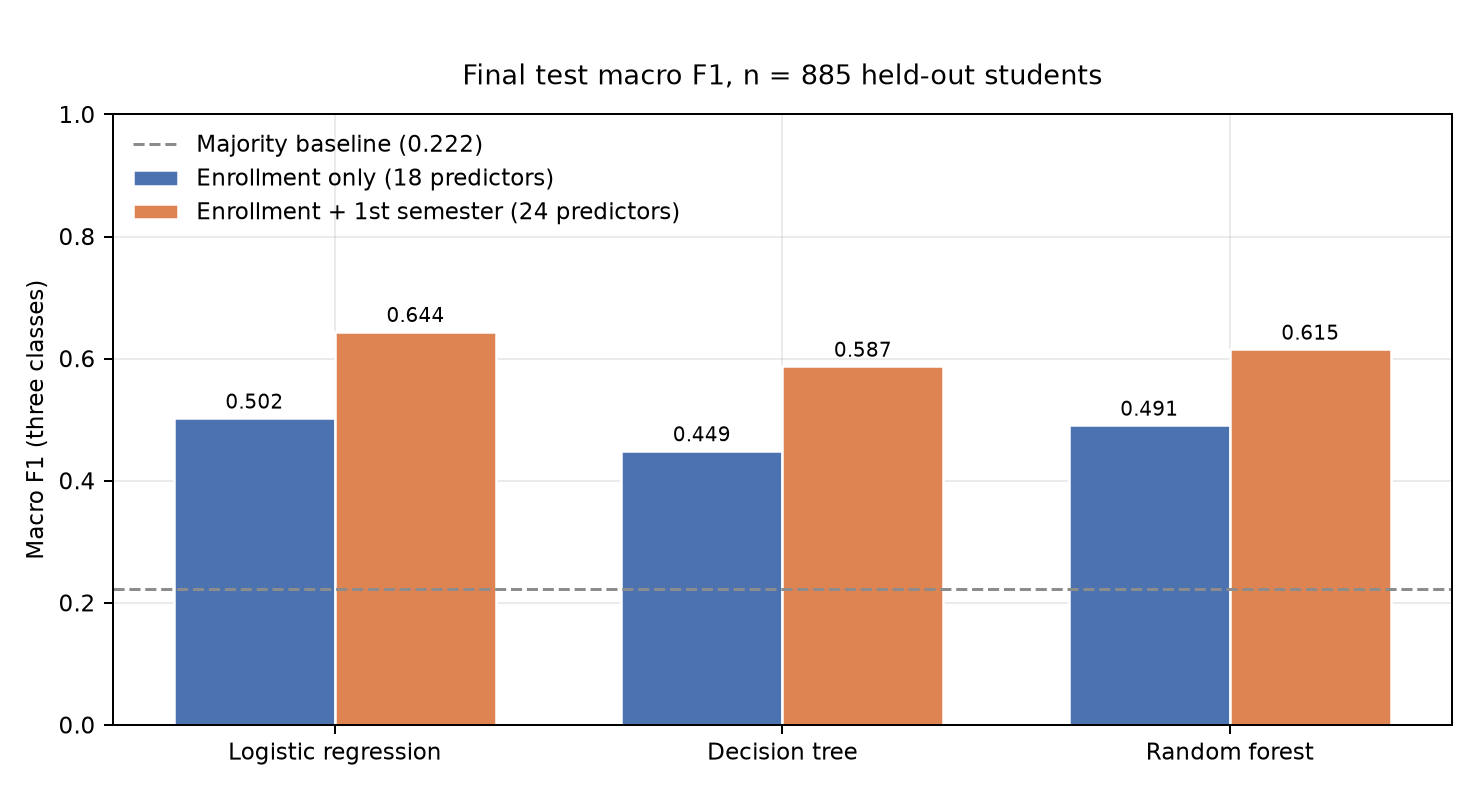
\includegraphics[width=\textwidth,height=0.43\textheight,keepaspectratio]{01_test_macro_f1_by_model.png}
\caption{Test macro-F1 for the six trained pipelines and the majority baseline.}
\label{fig:macro-f1}
\end{figure}

\begin{figure}[H]
\centering
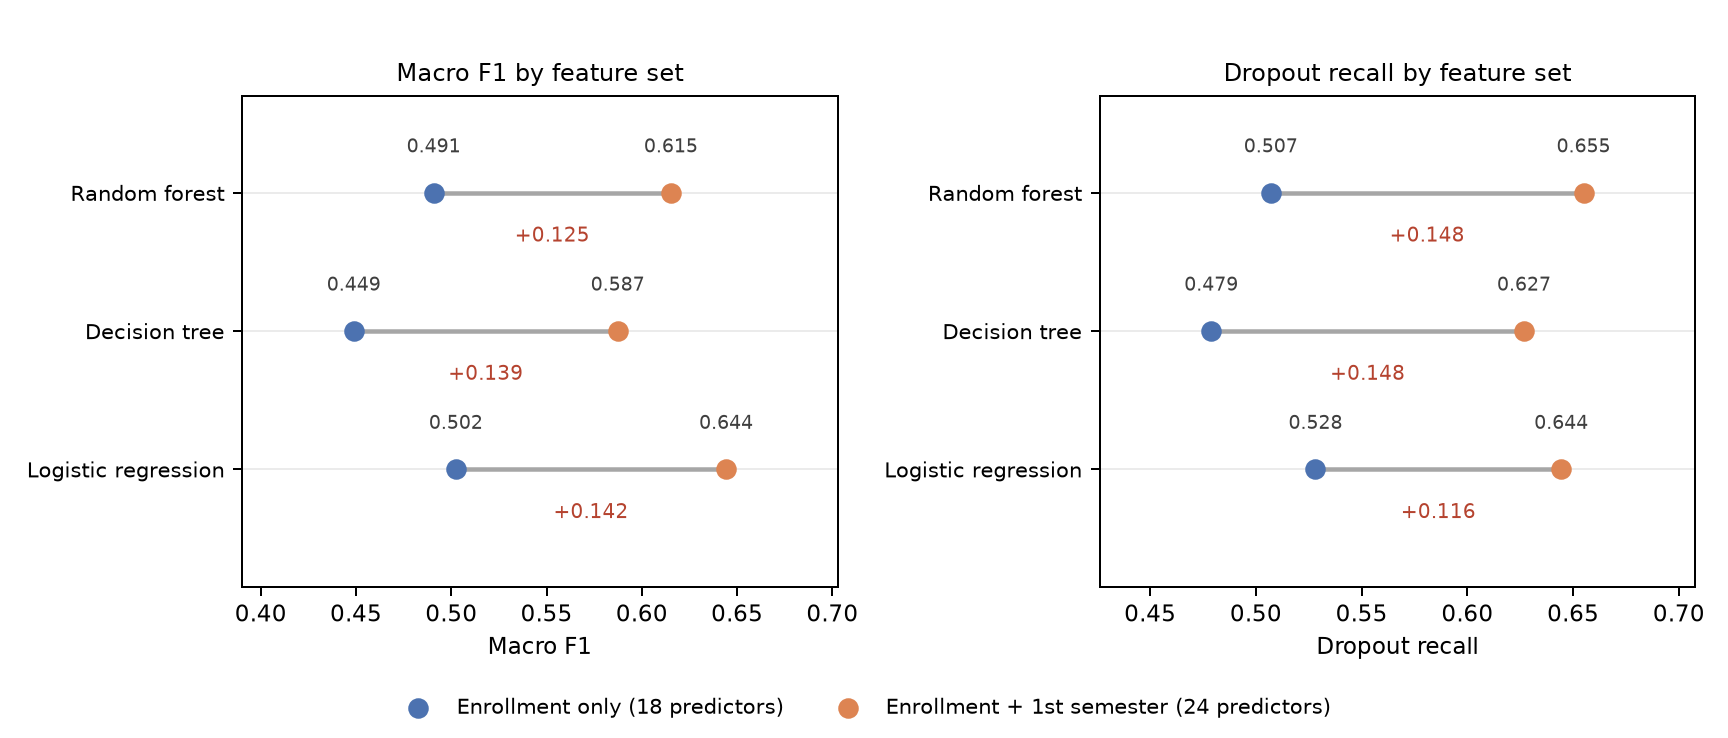
\includegraphics[width=\textwidth,height=0.43\textheight,keepaspectratio]{02_feature_set_gain.png}
\caption{Gain from adding the first-semester feature block.}
\label{fig:feature-gain}
\end{figure}

\subsection{Validation versus test ranking: does complexity pay off?}

This directly answers Research Question 2. Five of the six models score slightly lower on the
test set than in cross-validation, with an average drop of 0.017 macro-F1 — the expected mild
optimism from selecting hyperparameters on the same training rows. The notable result is at the
top of the ranking.

\textbf{Logistic regression performs at least as well as random forest.} On the 24-variable
feature set, logistic regression holds its validation score almost exactly (0.6444 $\to$ 0.6442),
while the random forest drops 0.030 (0.6449 $\to$ 0.6153). The resulting test gap of 0.029
favours logistic regression, but this margin is smaller than the fold-to-fold standard deviations
reported in cross-validation (logistic regression: $\pm$0.0159, random forest: $\pm$0.0172). It
must be treated as noise, not as a stable ranking.

\textbf{Statistical interpretation.} A single 885-row test set provides no confidence interval.
With 284 true Dropout cases, a swing of $\pm$0.02 macro-F1 is well inside sampling variation.
Proper significance testing would require multiple train-test splits or bootstrap resampling,
which was not performed here. The honest answer to Research Question 2 is: on the richer feature
set, logistic regression and random forest are \emph{statistically indistinguishable}; both are
clearly above the decision tree (0.5873) and far above the baseline (0.2221).

Because the random forest was designated as the representative model before test access, it
remains so for the interpretation analysis below. Changing that designation on the basis of
test results would be post-hoc selection.

\subsection{Class-level behaviour}

With 24 variables, Dropout precision ranges from 0.68 to 0.74 and Dropout recall from 0.63 to
0.65. Graduate is easier to identify (F1: 0.80--0.80). The \Enrolled{} class is consistently
weak across all models, with F1 ranging from 0.30 to 0.45.

Three factors explain why \Enrolled{} is hard to predict. First, there are only 159 \Enrolled{}
test cases (18\%), fewer than \Graduate{} (442) or \Dropout{} (284); balanced class weighting
helps but does not fully compensate. Second, ``still enrolled'' is a temporary state: at data
collection the student has not yet reached a terminal outcome, so the label conflates students
who will eventually graduate with those who will eventually drop out. Third, the available
features record past academic performance and demographics, but the factors that determine
whether an enrolled student stays — financial pressure, employment load, intention to transfer
— are not captured here.

The practical consequence is that the headline macro-F1 figure understates how uncertain the
models are for one of the three classes. The Figure~\ref{fig:confusion} confusion matrices make
this concrete. Among the 284 true \Dropout{} cases, the 24-variable logistic regression
misclassifies 32 as \Graduate{}; the random forest misclassifies 57 and the decision tree 70.
A support service can use the model to prioritise outreach, but should not interpret a non-flag
as confirmation that a student is safe.

\begin{figure}[H]
\centering
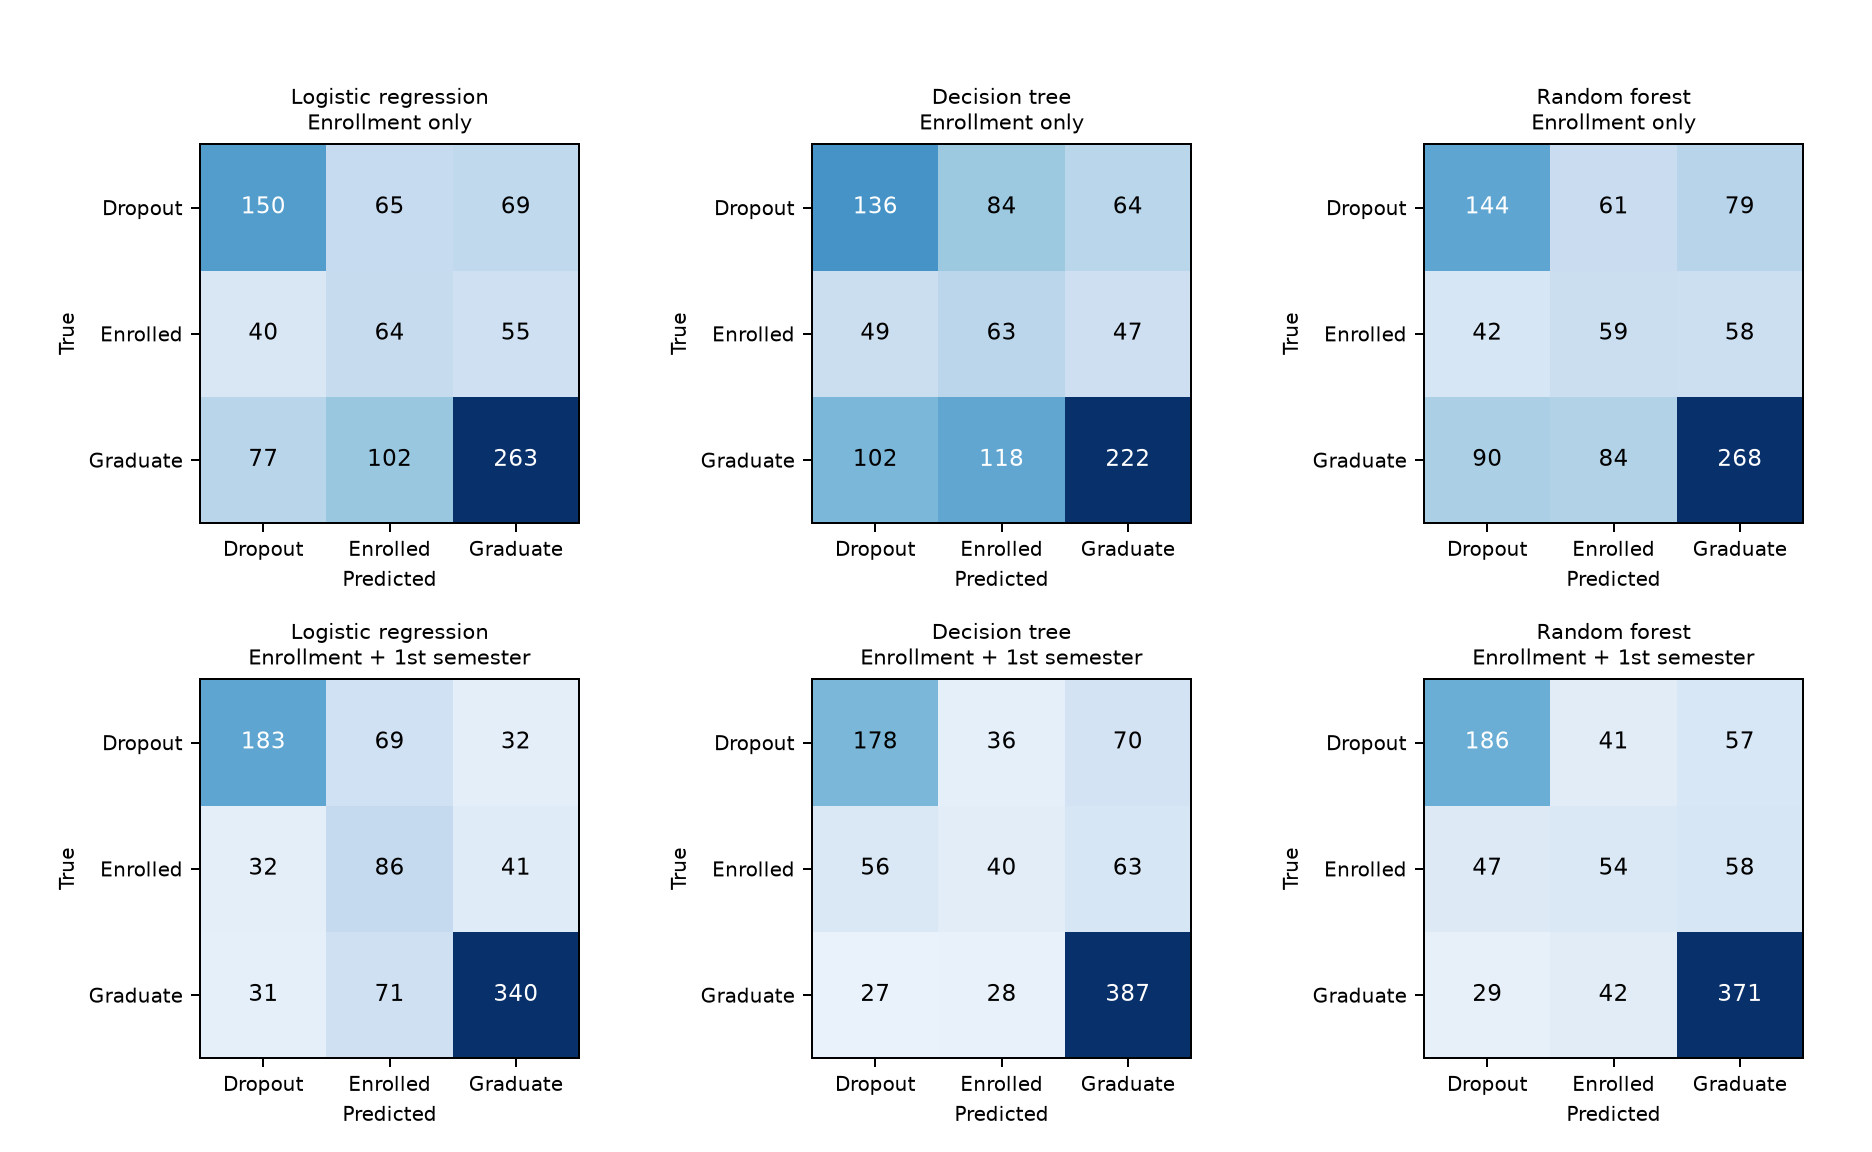
\includegraphics[width=\textwidth,height=0.55\textheight,keepaspectratio]{03_confusion_matrices.png}
\caption{Confusion matrices for the six trained pipelines on the held-out test set.}
\label{fig:confusion}
\end{figure}

The 24-variable logistic regression has a test log-loss of 0.7286. The results table does not
report log-loss for the tree models, and probability calibration was not evaluated in this project.
The available results therefore do not establish that model probabilities are calibrated risk
estimates.

\section{Model interpretation}

\subsection{Representative random forest: what drives prediction}

Permutation importance for the pre-specified 24-variable random forest (ten repeats, seed 42)
concentrates almost entirely on first-semester academic performance. The five largest effects are:

\begin{table}[H]
\centering
\caption{Top permutation importance features for the representative random forest (mean macro-F1
drop over 10 repeats, seed 42). Features below rank 5 are at or near the noise floor.}
\label{tab:importance}
\begin{tabular}{lrr}
\toprule
Feature & Mean macro-F1 drop & SD \\
\midrule
Curricular units 1st sem (approved) & 0.1078 & 0.0090 \\
Curricular units 1st sem (evaluations) & 0.0226 & 0.0083 \\
Curricular units 1st sem (grade) & 0.0160 & 0.0109 \\
Course & 0.0122 & 0.0083 \\
Mother's qualification & 0.0055 & 0.0064 \\
\bottomrule
\end{tabular}
\end{table}

Approved units alone cause five times the macro-F1 drop of the next feature. Background
variables — nationality, marital status, parental occupation, special needs status — sit at or
below the noise floor. Some importances are slightly negative, which is normal when features are
correlated. The model's predictive signal is almost entirely in what happens academically in the
first term, not in who the student is at enrolment.

\begin{figure}[H]
\centering
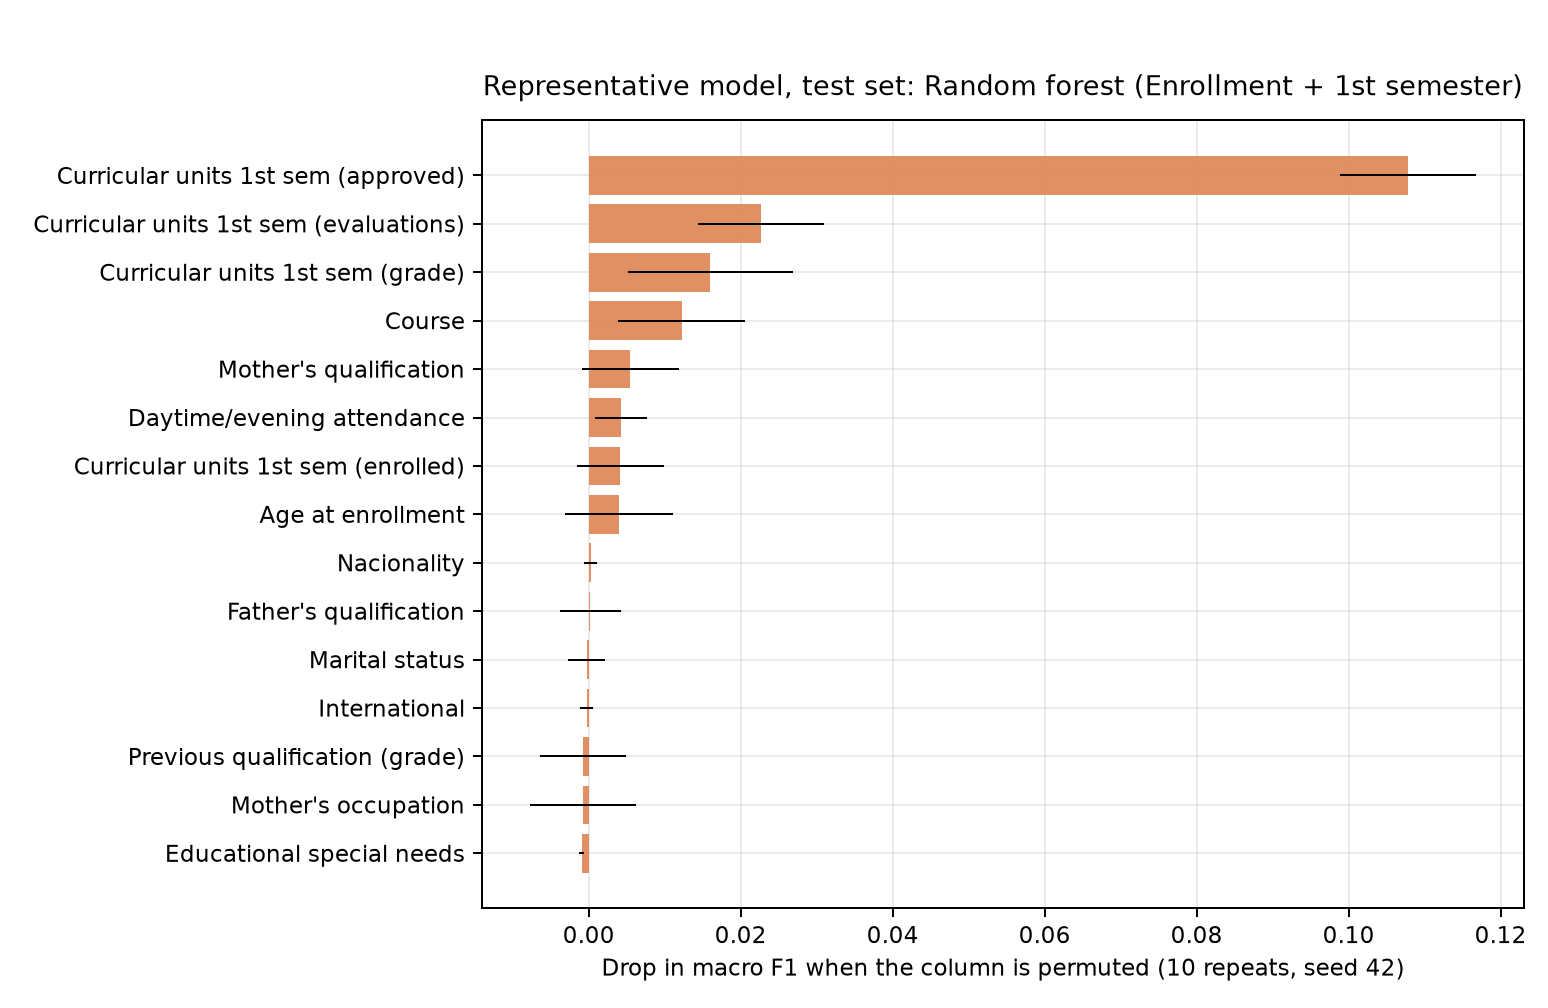
\includegraphics[width=\textwidth,height=0.48\textheight,keepaspectratio]{04_interpretation_random_forest.png}
\caption{Permutation importance for the pre-specified representative random forest (24-variable
feature set). Bars show mean macro-F1 decrease over 10 repeats; only features with positive mean
importance are shown.}
\label{fig:rf-importance}
\end{figure}

\subsection{Logistic regression: a human-readable signal}

The 24-variable logistic regression adds sign to the picture. The largest coefficient for the
\Dropout{} class is negative for approved first-semester units ($-1.77$): more approvals protect
against dropout. The number of units enrolled ($+0.85$) and credited ($+0.44$) push in the
opposite direction, and first-semester grade is also protective ($-0.34$). Age at enrolment
carries a small positive dropout coefficient ($+0.19$).

The pattern reads plainly: \textbf{students who register for many units but convert few into
approvals are the ones the model flags.} This is an observable academic behaviour during the
first term, and it gives an advising service something concrete to act on. A student enrolled in
six units with zero approvals by week eight is behaving very differently from one who has approved
all six, and that difference dominates everything else in the model.

\begin{figure}[H]
\centering
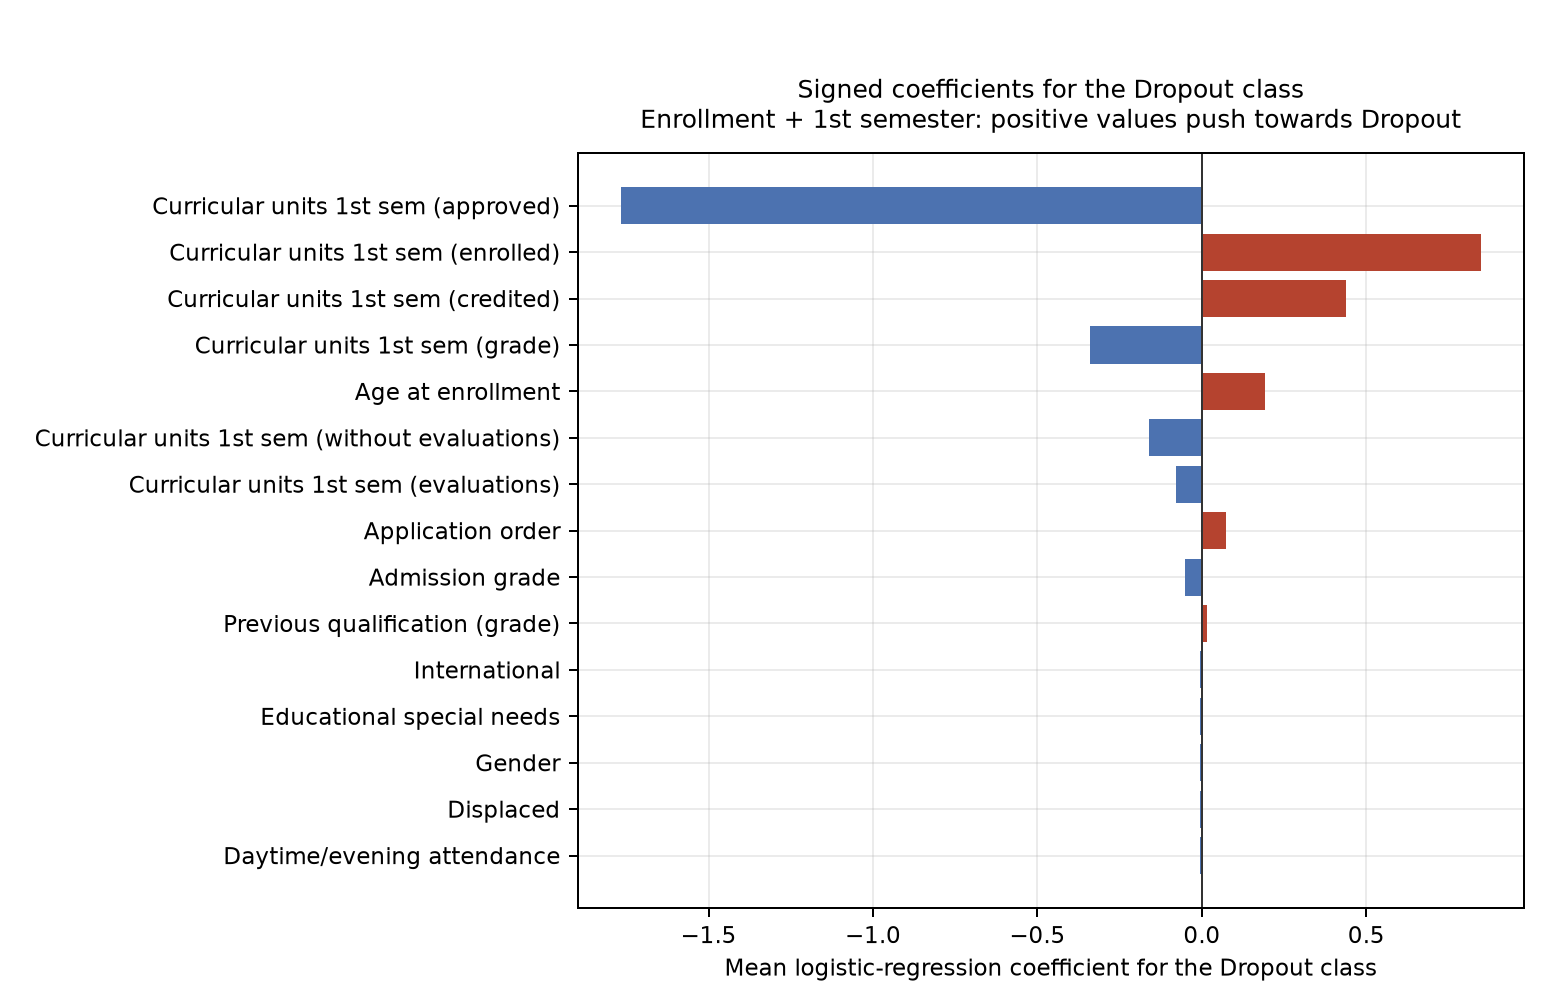
\includegraphics[width=\textwidth,height=0.48\textheight,keepaspectratio]{05_interpretation_logistic_regression.png}
\caption{Signed \Dropout{}-class coefficients for the 24-variable logistic regression. Negative
coefficients (approved units, grade) reduce dropout probability; positive coefficients (enrolled
units, credited units, age) increase it.}
\label{fig:logistic-coefficients}
\end{figure}

Two caveats apply. These are model-and-sample associations, not causal estimates: correlated
features can share or suppress each other's importance, and the enrolled/approved relationship
is partly mechanical (a student cannot approve units they never enrolled in). The figures also
describe this model on this test set; replication on other cohorts is needed before drawing
broader conclusions.

\section{Discussion}

\subsection{What the results show}

Enrolment-time information alone produces test macro-F1 of roughly 0.49 — better than the
majority baseline, but not by enough to justify targeted intervention on its own. Adding six
first-semester variables raises that to 0.62--0.64 across every model family, and the gain holds
on data the models never saw during tuning. Waiting a full term for first-semester records is
worth it.

Three results sharpen that headline. First, the simpler model is sufficient. Logistic regression
matches the random forest on the 24-variable set (0.6442 vs 0.6153, within fold-to-fold noise),
and its signed coefficients give advisors a readable account of why a student was flagged. The
ensemble offers no measurable operational advantage here. Second, the signal is behavioural. The
dominant feature by a factor of five is first-semester approved units; demographic and background
variables contribute negligibly. Students flagged for dropout risk are those who enrolled in many
units but converted few into approvals — an observable pattern during the first term, not a fixed
characteristic. Third, the \Enrolled{} class is the genuine limit of this approach. F1 of
0.30--0.45 across all models reflects a structural problem: ``still enrolled'' is an unresolved
state that the available features cannot distinguish from future graduation or future dropout.

\subsection{How these results could be used}

The results support one specific use case: a retrospective end-of-first-semester screening aid.
At that point, the 24-variable logistic regression flags roughly 380 of 885 students at 74\%
Dropout precision, of whom roughly 280 are true positives. An advising service can offer those
flagged students a review — tutoring, counselling, financial aid assessment, or course-load
discussion — without denying support to students who are not flagged.

A lighter-touch enrolment-time pass is possible in principle, but the weaker enrolment-only
performance means the first stage should be low-intensity. The main effort belongs at the end of
the first semester.

Any deployment requires five safeguards:
\begin{itemize}[leftmargin=*]
  \item \textbf{Human review.} No automated denial of support, admission, or financial aid on
  model predictions alone.
  \item \textbf{Outreach, not penalties.} Flagging means an offer of assistance; students not
  flagged can still request support.
  \item \textbf{Fairness audit.} The model uses age, nationality, gender, and parental
  background as inputs, so flagging rates must be checked by group before deployment.
  \item \textbf{Annual re-training.} Cohort composition and institutional policies change over
  time; models should be retrained and revalidated regularly.
  \item \textbf{Probability calibration.} A test log-loss of 0.7286 for logistic regression
  does not establish calibrated probabilities. Tree-model leaf proportions should not be used as
  risk scores without recalibration.
\end{itemize}

\subsection{What this study does not establish}

The comparison measures predictive association at two information points. It does not show that
first-semester performance causes dropout, and it does not measure whether targeted support
actually retains students. Those questions require a different design — a randomised or
quasi-experimental study that compares outcomes for supported versus unsupported students. The
present work provides the predictive signal; the intervention efficacy is a separate question.

\section{Limitations and future directions}

\begin{enumerate}[leftmargin=*]
  \item \textbf{Single held-out split.} One 885-row test set provides no confidence interval;
  with 284 true Dropout cases, a swing of $\pm$0.02 macro-F1 is within sampling noise. Future
  work should use nested cross-validation or bootstrap resampling to quantify uncertainty.

  \item \textbf{Weak middle class.} The 159 \Enrolled{} test cases yield F1 of 0.30--0.45. This
  reflects definitional ambiguity (``still enrolled'' conflates eventual graduates with eventual
  dropouts) and feature insufficiency (no data on financial pressure, employment load, or
  intention to transfer). Adding such features and using cost-sensitive learning could improve
  this class.

  \item \textbf{Retrospective timing.} First-semester variables become available only after a
  full term. The dataset contains no individual withdrawal dates, so the comparison is a
  retrospective snapshot, not a real-time alert. Dynamic tracking at multiple checkpoints within
  a semester would strengthen operational usefulness.

  \item \textbf{Institutional scope.} One Portuguese polytechnic, 2008--2019 cohorts. External
  validation on other institutions and countries is needed before any generalization claim.

  \item \textbf{Probability calibration.} Calibration was not evaluated. Logistic regression
  probabilities should be assessed with calibration curves; tree-model leaf proportions must not
  be used as risk scores without recalibration.

  \item \textbf{Outcome definition.} The \Dropout{} label is institution-specific. A student
  recorded as Dropout may have transferred and graduated elsewhere; the label is not a measure of
  lifetime educational attainment.

  \item \textbf{Causal and fairness gaps.} The model uses age, nationality, gender, and parental
  background as inputs. Flagging-rate audits by group are required before deployment. Estimating
  whether support interventions actually retain students requires a randomised or
  quasi-experimental study; the present work measures predictive signal only.
\end{enumerate}

\section{Conclusion}

This project asked one question: does adding first-semester academic records to enrolment-time
information meaningfully improve how well we can classify students as \Dropout{}, \Enrolled{},
or \Graduate{}? The answer is yes, consistently. Test macro-F1 rises by 0.125--0.142 across
logistic regression, decision tree, and random forest, on data the models never saw during
tuning. Enrolment-only models are too weak for targeted support; first-semester models are
substantially better, and waiting a full term for first-semester data is justified.

Two results matter beyond that headline. The simpler model is sufficient: logistic regression
matches the random forest, and its coefficients make the prediction readable — students who enrol
in many units but approve few are the ones flagged. That is an observable behaviour during the
first term, which an advising service can act on. And one class remains hard: the models cannot
reliably separate students who are still enrolled from those who will graduate or drop out, so
deployment should be honest about that limit.

The models are best used as a retrospective end-of-first-semester screening aid, with human
review, non-punitive outreach, and regular fairness audits. They support prioritising who to
contact; they do not justify automated decisions about who receives or loses support.

\section*{Data and code availability}

The data-processing, model-training, and evaluation scripts are stored in the project repository.
The exact commands, configuration files, frozen model paths, output tables, and environment notes
are listed in Appendix~\ref{app:code}. The source dataset is distributed by the UCI Machine
Learning Repository under CC BY 4.0; the repository retains its source citation and provenance
metadata.

\appendix
\section{Team contributions}
\label{app:contributions}

This appendix documents the division of work, deliverables, and verification records for all five
team members.

\subsection{Member A (Ruxuan ZHOU): Data preparation and experimental protocol}

Member A downloaded and preprocessed the UCI raw dataset, designed the fixed experimental protocol
(random seed, stratification strategy, and leakage controls), defined the 18-variable and
24-variable feature sets with documented exclusion criteria, and generated the split manifest and
configuration files. Verification passed 23/23 delivery checks.

\noindent\textit{Deliverables:}
\begin{itemize}[leftmargin=*,noitemsep,topsep=2pt]
  \item \path{data/processed/students.csv} (4,424 rows; checksums recorded in \path{data/manifest.json})
  \item \path{data/splits/split_manifest.csv} (\texttt{row\_id}, \texttt{dataset\_split}, \texttt{cv\_fold} assignments)
  \item \path{configs/protocol.json} and \path{configs/feature_sets.json}
  \item \path{src/A_data/prepare_data.py} and \path{src/A_data/verify_A.py}
  \item \path{docs/handoffs/A.md}
\end{itemize}

\subsection{Member B (Mingxi ZHU): Model training and hyperparameter tuning}

Member B implemented training pipelines for logistic regression, decision tree, and random forest
models, ran five-fold stratified cross-validation grid search on the training split, froze all six
model pipelines plus the majority-class baseline prior to test access, and pre-specified the
24-variable random forest as the representative model for interpretation. Verification passed 16/16
delivery checks, with all 35 validation folds independently recomputed to within $10^{-12}$.

\noindent\textit{Deliverables:}
\begin{itemize}[leftmargin=*,noitemsep,topsep=2pt]
  \item \path{src/B_models/train_models.py}, \path{src/B_models/verify_B.py},\\
  \path{src/B_models/test_b_models.py}
  \item \path{models/*.joblib} (six frozen model pipelines plus majority baseline)
  \item \path{results/B_validation/cv_metrics.csv}, \path{selected_params.json},\\
  \path{model_catalog.json}
  \item \path{docs/handoffs/B.md}
\end{itemize}

\subsection{Member C (Boyi WEI): Final evaluation and interpretation}

Member C applied the frozen pipelines to the held-out test split in a one-shot evaluation, computed
macro-F1, class-level precision and recall, accuracy, and log-loss, generated all five
interpretation figures, and computed permutation importance for the pre-specified representative
random forest. Verification passed 14/14 delivery checks; the prediction table contains 6,195 rows
(885 test students $\times$ 7 pipelines), and summary metrics recompute from stored predictions
within a maximum absolute error of $8.88 \times 10^{-16}$.

\noindent\textit{Deliverables:}
\begin{itemize}[leftmargin=*,noitemsep,topsep=2pt]
  \item \path{src/C_evaluation/evaluate_models.py} and \path{src/C_evaluation/verify_C.py}
  \item \path{results/C_final/test_metrics.csv} (seven model-level summary rows evaluated on 885 test students)
  \item \path{results/C_final/test_predictions.csv} (6,195 prediction and probability rows)
  \item \path{results/C_final/figures/*.png} (five visualisation figures)
  \item \path{results/C_final/permutation_importance_representative.csv},\\
  \path{results/C_final/logistic_dropout_coefficients.csv}, and \path{results/C_final/findings.md}
  \item \path{docs/handoffs/C.md}
\end{itemize}

\subsection{Member D (Mengqi YAN): Report integration and documentation}

Member D integrated technical materials from Members A, B, and C into the final report, drafted the
project proposal and reproducibility appendix, cross-checked reported figures against Member C's
output files, compiled references, and ensured adherence to experimental reporting standards.

\noindent\textit{Deliverables:}
\begin{itemize}[leftmargin=*,noitemsep,topsep=2pt]
  \item \path{docs/report/report.pdf} (this document)
  \item \path{docs/report/main_report.tex}, \path{docs/report/code_appendix.tex},\\
  \path{docs/report/references.bib}
  \item \path{docs/proposal/proposal.pdf}
\end{itemize}

\subsection{Member E (Yushu WU): Presentation and dissemination}

Member E cross-checked the report's numerical results against Member C's evaluation outputs (including
dropout counts, precision, and recall), prepared the presentation slides incorporating the report's
key figures, authored the bilingual English--Chinese presentation script for all five members,
coordinated and completed the recorded group presentation, and designed the A0 project poster.

\noindent\textit{Deliverables:}
\begin{itemize}[leftmargin=*,noitemsep,topsep=2pt]
  \item \path{recording/Student-Dropout-Prediction.mp4}
  \item \texttt{slides/Team-Zero bias hero-PPT.pptx}
  \item \texttt{slides/Team-Zero bias hero-Poster.pptx}
  \item \texttt{slides/Team-Zero bias hero-Script.docx}
\end{itemize}

\section{Reproducibility and code appendix}
\label{app:code}

\subsection{Repository layout}

The full codebase, configurations, frozen models, evaluation outputs, and presentation materials are
hosted in a public GitHub repository:
\begin{itemize}[leftmargin=*,noitemsep,topsep=2pt]
  \item \textbf{Repository:} \url{https://github.com/GeorgeZhou888/DSC5001-Student-Dropout-Prediction}
  \item \textbf{Branch:} \texttt{main}
  \item \textbf{Data licence:} The UCI source dataset is licensed under CC BY 4.0; no separate licence is specified for the project code.
\end{itemize}

Key project files are organised by stage:
\begin{itemize}[leftmargin=*,noitemsep,topsep=2pt]
  \item Data preparation: \path{src/A_data/prepare_data.py}, \path{src/A_data/verify_A.py}.
  \item Protocol and feature definitions: \path{configs/protocol.json}, \path{configs/feature_sets.json}.
  \item Model training and checks: \path{src/B_models/train_models.py},\\
  \path{src/B_models/verify_B.py}, \path{src/B_models/test_b_models.py}.
  \item Final evaluation and checks: \path{src/C_evaluation/evaluate_models.py},\\
  \path{src/C_evaluation/verify_C.py}.
  \item Final outputs: \path{results/C_final/test_metrics.csv},\\
  \path{results/C_final/test_predictions.csv}, interpretation CSVs, and figures in \path{results/C_final/figures/}.
\end{itemize}

\subsection{Environment}

All three computational stages ran under Python 3.14.x with dependencies pinned in\\
\path{environment/requirements-lock.txt}. The recorded runs used different operating systems and
patch versions: Stage A used Python 3.14.6 on macOS ARM64, Stage B used Python 3.14.5 on Windows
AMD64, and Stage C used Python 3.14.3 on Windows AMD64. The run manifests preserve these exact
runtime details rather than treating the environments as identical.

\subsection{Commands}

All commands below are executed from the repository root and are platform-neutral apart from the
local Python executable name.

\begin{lstlisting}[language=bash,caption={Data preparation and verification}]
python src/A_data/prepare_data.py
python src/A_data/verify_A.py
python src/A_data/verify_A.py --reproduce
\end{lstlisting}

\begin{lstlisting}[language=bash,caption={Model verification and pre-evaluation checks}]
python -m unittest discover -s src/B_models -p test_b_models.py -v
python src/B_models/verify_B.py --recheck-cv
python src/C_evaluation/evaluate_models.py --check
python src/C_evaluation/verify_C.py
\end{lstlisting}

The held-out test evaluation was executed once using the frozen Stage B pipelines, with all outputs
archived under \path{results/C_final/}:

\begin{lstlisting}[language=bash,caption={One-shot held-out test evaluation}]
python src/C_evaluation/evaluate_models.py
\end{lstlisting}

By design, \path{evaluate_models.py} refuses to overwrite an existing output directory unless an
explicit override flag (\texttt{-\/-force}) is supplied, protecting the archived one-shot evaluation
results from accidental regeneration.

\subsection{Protocol summary}

\begin{table}[H]
\centering
\caption{Fixed analysis protocol.}
\label{tab:protocol}
\begin{tabular}{ll}
\toprule
Item & Setting \\
\midrule
Raw records & 4,424 \\
Train/test counts & 3,539 / 885 \\
Outer split & Stratified 80/20, seed 42 \\
Training validation & Five-fold stratified cross-validation \\
Feature sets & 18 enrolment variables; 24 enrolment plus semester-1 variables \\
Models & Logistic regression, decision tree, random forest \\
Baseline & Majority class \\
Selection metric & Macro-F1 \\
Test-set use & One final evaluation after model freezing \\
\bottomrule
\end{tabular}
\end{table}

\subsection{Provenance notes}

The final evaluation manifest (\path{results/C_final/run_manifest.json}) records the frozen Stage B
reference, input SHA-256 digests and accepted line-ending states, model hashes, output hashes,
runtime environment, and execution command. The Stage C verification report confirms 14 of 14 checks
passing: the archived prediction table holds 6,195 rows (885 test students across seven pipelines),
and every summary metric in \path{results/C_final/test_metrics.csv} recomputes directly from those
stored predictions, establishing internal consistency and full provenance for the final project
deliverables.


\bibliographystyle{plainnat}
\bibliography{references}

\end{document}
